\documentclass[MathsNotesBase.tex]{subfiles}

\date{\vspace{-6ex}}



\begin{document}

\searchableSubsection{Linear Algebra of Polynomials}{linear algebra, polynomials}{
	\bigskip\bigskip
	\newcommand\imgDir{\resourceDir/img/LinearAlgebraOfPolynomials_images}
	
	\subsubsection{Uniqueness of Polynomials}
	\bigskip
	\labeledProposition{Three points uniquely identify a quadratic polynomial.}{three_points_identify_quadratic}
	\begin{proof}
		Assume that there are two distinct quadratic polynomials ${ p(x),\, q(x) }$ that share 3 points. That is,
		\[ p(x_1) = q(x_1),\, p(x_2) = q(x_2),\, p(x_3) = q(x_3). \]
		Then we can define another quadratic polynomial ${ r(x) = p(x) - q(x) }$ with the property that,
		\[ r(x_1) = p(x_1) - q(x_1) = 0 = r(x_2) = r(x_3). \]
		In other words, $r(x)$ has 3 roots: ${ x_1,x_2,x_3 }$. But $r(x)$ is a quadratic polynomial and has a maximum of 2 roots. Therefore there is non such (nonzero) polynomial.
	\end{proof}

	\subsubsection{Uniqueness of Coefficients of Polynomials}\TODO{is this the best place for this?}
	\labeledTheorem{If a polynomial is identically zero (i.e. the zero function), then all coefficients are 0.}{identically-zero-polynomial-has-all-zero-coefficents}
	\begin{proof}
		An obvious way to prove this is to begin by assuming that we have a degree-$m$ polynomial,
		\[ p(x) = a_0 + a_1 x + \cdots + a_m x^m \]
		where any coefficients $a_i$ with ${ i < m }$ may be zero. Then we can reason that if $p(x)$ is zero for all ${ x \in \R{} }$ then its derivative $p'(x)$ must also be identically zero. In this way we can extend the implication to lower and lower degree polynomials by differentiation until $p^{(m)}$ is a degree zero polynomial,
		\[ p^{(m)}(x) = m!\, a_m = 0 \implies a_m = 0. \]
		But ${ a_m = 0 }$ contradicts the hypothesis that $p(x)$ is a degree-$m$ polynomial.\\
		
		Another (better?) proof is given in Linear Algebra Done Right as follows.\\
		
		Let
		\[ x = \frac{\abs{a_0} + \abs{a_1} + \cdots + \abs{a_{m-1}}}{\abs{a_m}} + 1 \]
		so that ${ x \geq 1 }$ and so ${ \abs{a_0} \leq \abs{a_0} x }$. Then, using the triangle inequality,
		\[ \abs{a_0 + a_1 x} \leq \abs{a_0} + \abs{a_1 x} \leq \abs{a_0 x} + \abs{a_1 x} = (\abs{a_0} + \abs{a_1}) x. \]
		Using induction with an inductive step,
		\begin{align*}
		&& \abs{a_0 + a_1 x + \cdots + a_{n-1} x^{n-1}} &\leq (\abs{a_0} + \cdots + \abs{a_{n-1}}) x^{n-1} \\
		&\implies & \abs{a_0 + a_1 x + \cdots + a_n x^n} &\leq \abs{a_0 + a_1 x + \cdots + a_{n-1} x^{n-1}} + \abs{a_n x^n}\\
		&&&\leq (\abs{a_0} + \cdots + \abs{a_{n-1}}) x^{n-1} + \abs{a_n} x^n \\
		&&&\leq (\abs{a_0} + \cdots + \abs{a_{n-1}} + \abs{a_n}) x^n
		\end{align*}
		we can deduce that
		\[ \abs{a_0 + a_1 x + \cdots + a_{m-1} x^{m-1}} \leq (\abs{a_0} + \cdots + \abs{a_{m-1}}) x^{m-1}. \]
		Now, 
		\begin{align*}
		\abs{a_m x^m} = \abs{a_m} x^m &= (\abs{a_m} x) x^{m-1} \\
		&= \left[\abs{a_m} \left(\frac{\abs{a_0} + \abs{a_1} + \cdots + \abs{a_{m-1}}}{\abs{a_m}} + 1\right)\right] x^{m-1}\\
		&= \left(\abs{a_0} + \abs{a_1} + \cdots + \abs{a_{m-1}} + \abs{a_m}\right) x^{m-1}.
		\end{align*}
		Therefore, combining with the previous result, we have,
		\[ \abs{a_0 + a_1 x + \cdots + a_{m-1} x^{m-1}} \leq (\abs{a_0} + \cdots + \abs{a_{m-1}}) x^{m-1} < \abs{a_m x^m}. \]
		We can now reason that,
		\begin{align*}
		&& \abs{a_0 + a_1 x + \cdots + a_{m-1} x^{m-1}} &<  \abs{a_m x^m} \\
		&\implies & a_0 + a_1 x + \cdots + a_{m-1} x^{m-1} &\neq -a_m x^m  &\sidecomment{} \\
		&\iff & a_0 + a_1 x + \cdots + a_{m-1} x^{m-1} + a_m x^m &\neq 0.
		\end{align*}
	\end{proof}

	\bigskip\bigskip
	\subsubsection{Lagrange Polynomials}
	\bigskip
	\begin{par}
	\begin{flushleft}
	If we look for quadratic polynomials, $p\left(x\right)$, that pass throught the 3 points (1, 3), (3, 1) and (5, 2):
	\end{flushleft}
	\end{par}
	
	\begin{center}
	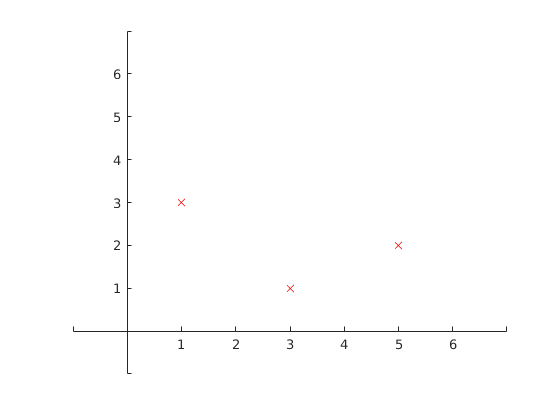
\includegraphics[width=\linewidth]{\imgDir/figure_0.png}
	\end{center}
	
	
	\begin{par}
	\begin{flushleft}
	Then the first has roots at $x=1,3$ and passes through the point (5, 2). So, we have:
	\end{flushleft}
	\end{par}
	
	\begin{par}
	$$p(1)=p(3)=0, p(5) = 2$$
	\end{par}
	
	\begin{par}
	\begin{flushleft}
	meaning that $\left(x-1\right)$ and $\left(x-3\right)$ are factors. Therefore,
	\end{flushleft}
	\end{par}
	
	\begin{par}
	$$\begin{array}{lcr}
	&p(x) &= \alpha(x-1)(x-3)\\
	&&= \alpha(x^2-4x+3)
	\end{array}$$
	\end{par}
	
	\begin{par}
	$$\begin{array}{lcr}
	&p(5)&=2 \\
	\Longrightarrow &\alpha(5^2-4(5) + 3) &= 2 \\
	\iff &8\alpha&=2\\
	\iff &\alpha &= \frac{1}{4}\\
	\end{array}$$
	\end{par}
	
	\begin{par}
	$$\therefore p(x) = \frac{1}{4}(x^2-4x+3)$$
	\end{par}
	
	
	\begin{center}
	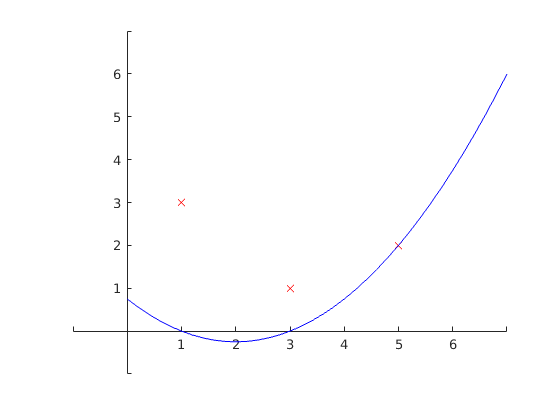
\includegraphics[width=\linewidth]{\imgDir/figure_1.png}
	\end{center}
	
	
	\begin{par}
	\begin{flushleft}
	The second has roots at $x=1,5$ and passes throught the point (3, 1):
	\end{flushleft}
	\end{par}
	
	\begin{par}
	$$\begin{array}{lcr}
	&p(x) &= \alpha(x-1)(x-5)\\
	&&= \alpha(x^2-6x+5)
	\end{array}$$
	\end{par}
	
	\begin{par}
	$$\begin{array}{lcr}
	&p(3)&=1 \\
	\Longrightarrow &\alpha(3^2-6(3) + 5) &= 1 \\
	\iff &-4\alpha&=1\\
	\iff &\alpha &= -\frac{1}{4}\\
	\end{array}$$
	\end{par}
	
	\begin{par}
	$$\therefore p(x) = -\frac{1}{4}(x^2-6x+5)$$
	\end{par}
	
	
	\begin{center}
	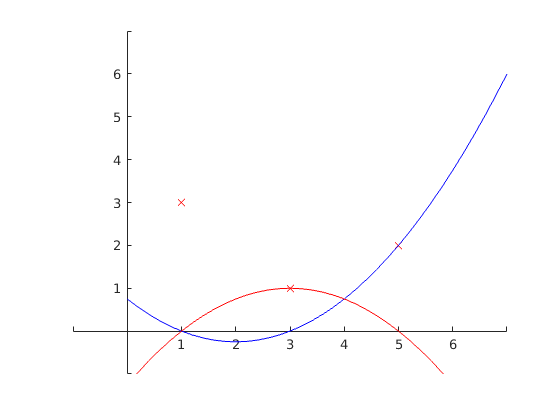
\includegraphics[width=\linewidth]{\imgDir/figure_2.png}
	\end{center}
	
	
	\begin{par}
	\begin{flushleft}
	The third has roots at $x=3,5$ and passes through the point (1, 3):
	\end{flushleft}
	\end{par}
	
	\begin{par}
	$$\begin{array}{lcr}
	&p(x) &= \alpha(x-3)(x-5)\\
	&&= \alpha(x^2-8x+15)
	\end{array}$$
	\end{par}
	
	\begin{par}
	$$\begin{array}{lcr}
	&p(1)&=3 \\
	\Longrightarrow &\alpha(1^2-8(1) + 15) &= 3 \\
	\iff &8\alpha&=3\\
	\iff &\alpha &= \frac{3}{8}\\
	\end{array}$$
	\end{par}
	
	\begin{par}
	$$\therefore p(x) = \frac{3}{8}(x^2-8x+15)$$
	\end{par}
	
	
	\begin{center}
	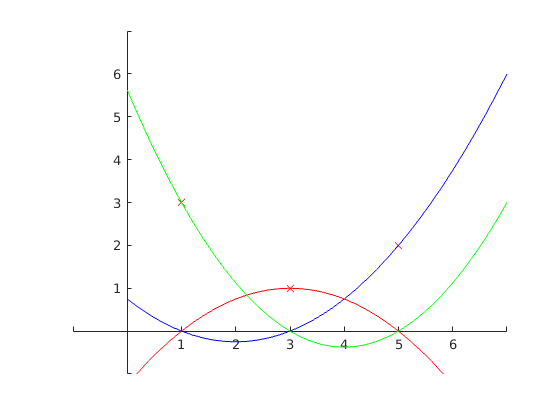
\includegraphics[width=\linewidth]{\imgDir/figure_3.png}
	\end{center}
	
	
	\begin{par}
	\begin{flushleft}
	Adding them together we get,
	\end{flushleft}
	\end{par}
	
	\begin{par}
	$$\begin{array}{lcr}
	\;\;\;\;\; \frac{1}{4}(x^2-4x+3) - \frac{1}{4}(x^2-6x+5) + \frac{3}{8}(x^2-8x+15) \\[8pt]
	= (\frac{1}{4}  - \frac{1}{4} + \frac{3}{8})x^2 + (-1 + \frac{3}{2} - 3)x + (\frac{3}{4} - \frac{5}{4} + \frac{45}{8}) \\[8pt]
	= \;\; \frac{3}{8}x^2 - \frac{5}{2}x + \frac{41}{8} 
	\end{array}$$
	\end{par}
	
	
	\begin{center}
	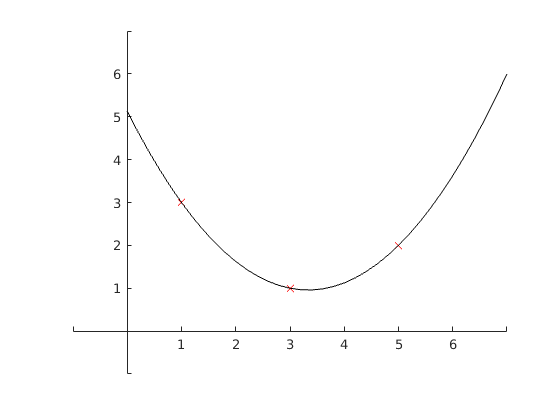
\includegraphics[width=\linewidth]{\imgDir/figure_4.png}
	\end{center}

	\bigskip\bigskip
	\subsubsection{Matrix approach}
	\bigskip
	We are looking for the unique quadratic polynomial ${ p(x) = \alpha_1x^2 + \alpha_2x + \alpha_3 }$ that satisfies
	\[ p(1)=3,\, p(3)=1,\, p(5)=2 \]
	so this gives us the simultaneous equations:
	\begin{align*}
	&& \alpha_1 + \alpha_2 + \alpha_3 &= 3 \\
	&& 9\alpha_1 + 3\alpha_2 + \alpha_3 &= 1 \\
	&& 25\alpha_1 + 5\alpha_2 + \alpha_3 &= 2 \\
	\end{align*}
	which can be expressed as a matrix equation,
	\[ 
		\begin{bmatrix}
		1 & 1 & 1\\
		9 & 3 & 1\\
		25 & 5 & 1
		\end{bmatrix}
		\begin{bmatrix}\alpha_1\\\alpha_2\\\alpha_3\end{bmatrix} 
		=
		\begin{bmatrix}3\\1\\2\end{bmatrix}.
	\]
	Now,
	\[ 
		\inv{\begin{bmatrix}
			1 & 1 & 1\\
			9 & 3 & 1\\
			25 & 5 & 1
			\end{bmatrix}} 
		=
		\begin{bmatrix}
		1/8  & -1/4 & 1/8\\
		-1   & 3/2  & -1/2\\
		15/8 & -5/4 & 3/8
		\end{bmatrix}
	\]
	so we have,
	\[
		 \begin{bmatrix}\alpha_1\\\alpha_2\\\alpha_3\end{bmatrix} 
		 =
		 \begin{bmatrix}
		 1/8  & -1/4 & 1/8\\
		 -1   & 3/2  & -1/2\\
		 15/8 & -5/4 & 3/8
		 \end{bmatrix}
		 \begin{bmatrix}3\\1\\2\end{bmatrix}
		 =
		 \begin{bmatrix}
		 3/8 - 1/4 + 1/4\\
		 -3 + 3/2 - 1\\
		 45/8 - 5/4 + 3/4
		 \end{bmatrix}
		 =
		 \begin{bmatrix}3/8\\-5/2\\41/8\end{bmatrix}.
	\]
	Therefore ${ p(x) = (3/8)x^2 + (-5/2)x + (41/8) }$.
	
	\bigskip\bigskip
	\subsubsection{Unified view}
	\bigskip
	Consider each of the component lagrange polynomials:
	\begin{itemize}
		\item{${ p_1(x) = \frac{1}{4}(x^2-4x+3) = (1/4)x^2 - x + (3/4) }$
			\[ \V{p}_1 = \begin{bmatrix}1/4\\-1\\3/4\end{bmatrix} \eqand 
				\begin{bmatrix}
				1 & 1 & 1\\
				9 & 3 & 1\\
				25 & 5 & 1
				\end{bmatrix}
				\V{p}_1 =
				\begin{bmatrix}
				1/4 - 1 + 3/4\\
				9/4 - 3 + 3/4\\
				25/4 - 5 + 3/4
				\end{bmatrix} =
				\begin{bmatrix}0\\0\\2\end{bmatrix}.
			\]
		}
		\item{${ p_2(x) = -\frac{1}{4}(x^2-6x+5) }$
			\[ \V{p}_2 = \begin{bmatrix}-1/4\\3/2\\-5/4\end{bmatrix} \eqand 
				\begin{bmatrix}
				1 & 1 & 1\\
				9 & 3 & 1\\
				25 & 5 & 1
				\end{bmatrix}
				\V{p}_2 =
				\begin{bmatrix}
				-1/4 + 3/2 - 5/4\\
				-9/4 + 9/2 - 5/4\\
				-25/4 + 15/2 - 5/4
				\end{bmatrix} =
				\begin{bmatrix}0\\1\\0\end{bmatrix}.
			\]
		}
		\item{${ p_3(x) = \frac{3}{8}(x^2-8x+15) }$
			\[ \V{p}_3 = \begin{bmatrix}3/8\\-3\\45/8\end{bmatrix} \eqand 
				\begin{bmatrix}
				1 & 1 & 1\\
				9 & 3 & 1\\
				25 & 5 & 1
				\end{bmatrix}
				\V{p}_3 =
				\begin{bmatrix}
				3/8 - 3 + 45/8\\
				27/8 - 9 + 45/8\\
				75/8 - 15 + 45/8
				\end{bmatrix} =
				\begin{bmatrix}3\\0\\0\end{bmatrix}.
			\]
		}
	\end{itemize}
	So,
	\[ \begin{bmatrix}
		1 & 1 & 1\\
		9 & 3 & 1\\
		25 & 5 & 1
		\end{bmatrix}
		(\V{p}_1 + \V{p}_2 + \V{p}_3)
		 = 
		\begin{bmatrix}0\\0\\2\end{bmatrix} + \begin{bmatrix}0\\1\\0\end{bmatrix} + \begin{bmatrix}3\\0\\0\end{bmatrix}
		= 
		\begin{bmatrix}3\\1\\2\end{bmatrix}.
	\]
}

\end{document}
